\documentclass{beamer}
\usetheme{afm}

\title{Portfolio Optimization}
\author{Matteo Sani - \href{mailto:matteo.sani@unisi.it}{matteo.sani@unisi.it}}

\begin{document}
\begin{frame}[plain]
	\maketitle
\end{frame}

\begin{frame}{Main Concepts and Some Notation}
  \begin{itemize}
  \item Portfolio optimization models look for the optimal way to make investments. 
  \item Usually investors expect either a maximum return for a given level of risk or a given return for a minimum risk so these models are typically based on two criteria: \emph{maximization of the expected return and/or minimization of the risk}.
  \item A portfolio is characterized by the \emph{weights} ($w_i$), representing the fraction of the total wealth invested in each asset.
  \item Few definitions:
    \begin{itemize}
    \item expected return: $\mathbb{E}(R_{p}) = \sum _{i}w_{i} \mathbb{E}(R_{i}) = \mathbf{w}\cdot \mathbf{R}$ (with $\sum_{i}w_i = 1$ and $0 \le w_i \le 1$);
    \item portfolio return variance: $ \sigma _{p}^{2} = \sum _{i}\sum _{j}w_{i}w_{j}\sigma _{ij} = \mathbf{w}^T\Sigma\mathbf{w}$ where $\Sigma = \sigma _{ij}=\sigma _{i}\sigma _{j}\rho _{ij}$ is the covariance, $\rho_{ij}$ is the correlation coefficient;
    \item portfolio standard deviation: $ \sigma _{p}= \sqrt{\sigma _{p}^{2}}$.
    \end{itemize}
  \end{itemize}
\end{frame}

\begin{frame}[fragile]{Definitions in \texttt{python}}
\begin{ipython}
import numpy as np

w = np.array([0.1, 0.2, 0.5, 0.05, 0.1])
R = np.array([0.239188, 0.415127, 0.263797, 0.172818, 0.528046])
Sigma = np.array([[0.051902, 0.025037, 0.025737, 0.022454, 0.027760],
                  [0.025037, 0.085839, 0.041025, 0.039501, 0.048412],
                  [0.025737, 0.041025, 0.069550, 0.036127, 0.044528],
                  [0.022454, 0.039501, 0.036127, 0.051797, 0.040390],
                  [0.027760, 0.048412, 0.044528, 0.040390, 0.178298]])

ret = R.dot(w) # np.dot(R, w)
var = w.T.dot(Sigma.dot(w)) # np.dot(w.T, np.dot(Sigma, w))
std = np.sqrt(var)
print (f"Portfolio return {ret:.4f}")
print (f"Portfolio variance {var:.4f}")
print (f"Portfolio std. dev. {std:.4f}")
\end{ipython}
\begin{ioutput}
Portfolio return 0.3003
Portfolio variance 0.0452
Portfolio std. dev. 0.2126
\end{ioutput}
\end{frame}

\begin{frame}{Modern Portfolio Theory (MPT)}
  \begin{itemize}
  \item Any theory concerning portfolio management aims to provide an "optimal" way to determine weights.
  \item MPT model assumes an investor usually consider \emph{expected return and variance in return}.
  \item Markowitz intuition was to estimate investment risk through portfolio variance i.e. it measures the variability in realized return around the expected return.  
  \item The latter characterizes not only the individual variability of the return on each investment, but also how each investment’s return tends to move with other investments. 
  \end{itemize}
\end{frame}

\begin{frame}{Modern Portfolio Theory}
  \begin{block}{Efficient Portfolios}
    There is no precise way for an investor to determine the “correct” trade off between risk and return. Generally higher expected return has to be paid with higher risk. Portfolio weights $w_i$ should be chosen such that it yields the highest return for a certain level of risk (or equivalently the lowest risk for a certain level of return)
    \begin{equation*}
      \max\{R_P\} = \underset{\mathbf{w}}{\max}\{\mathbf{w}\cdot\mathbf{R}\}\quad\textrm{subjected to }\mathbf{w}^T\Sigma\mathbf{w} = (\sigma_P^{target})^2
    \end{equation*}
or
    \begin{equation*}
      \min\{\sigma_P^2\}= \underset{\mathbf{w}}{\min}\{\mathbf{w}^T\Sigma\mathbf{w}\}\quad\textrm{subjected to }\mathbf{w}\cdot\mathbf{R} = R_P^{target}
    \end{equation*}
  \end{block}
\end{frame}

\begin{frame}{Efficient Frontier}
  The \emph{efficient frontier} consists of the set of all efficient portfolios that have the lowest level of risk for each expected return.
  \begin{figure}[h]
    \begin{center}
      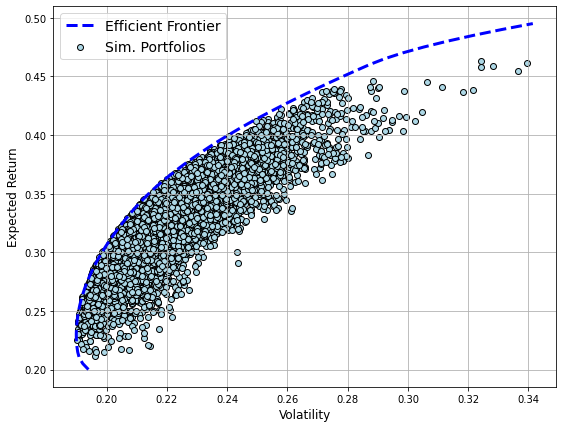
\includegraphics[width=0.4\linewidth]{efficient_frontier}
    \end{center}
  \end{figure}
  The efficient frontier is a parabola since the quadratic dependence of the variance to the portfolio wieghts.
\end{frame}

\begin{frame}{Criticism to Markowitz Theory}
  \begin{itemize}
  \item The portfolio weights tend to be extremely sensitive to very small changes in the expected returns.
  \item For example, even a small increase in the expected return of just one asset can dramatically alter the optimal composition of the entire portfolio.
  \item The presence of heavy tails in the return distributions can result in significant errors in covariance estimates as well (return normality assumption).
  \end{itemize}
\end{frame}

\begin{frame}{Portfolio with Risk-Free Asset}
  \begin{itemize}
  \item When one of the asset of the portfolio is risk free, then the efficient frontier has a particularly simple form: the \emph{capital allocation line} (CAL). 
  \item Consider a portfolio with two assets: one risk-free with $\mathbb{E}[R_f] = 3\%$ (e.g. treasury bill) and one risky (e.g. a stock) with $\mathbb{E}[R_r] = 10\%$ and standard deviation $\sigma_r = 20\%$.
  \item The question that needs to be answered for any individual investor is how much to invest in each of these assets
    \begin{equation*}
      \mathbb{E}[R_p] = \mathbb{E}[R_f]\cdot w_f + \mathbb{E}[R_r] \cdot ( 1 - w_f )
    \end{equation*}
    where $w_f$ is the relative allocation to the risk-free asset.
    \begin{equation*}
      \sigma_p = ( 1 - w_f ) \cdot \sigma_r
    \end{equation*}
  \end{itemize}
\end{frame}

\begin{frame}{Portfolio with Risk-Free Asset}
  \begin{itemize}
  \item If $w_f = 1$ the expected return would be 3\% and the risk of the portfolio would be 0\%. 
  \item If $w_f = 0$ would give an investor an expected return of 10\% and a portfolio risk of 20\%. 
  \item If $w_f=0.25$:
    \begin{equation*}
      \begin{gathered}
      \mathbb{E}[R_p] = ( 3\% \cdot 25\% ) + ( 10\% \cdot 75\% ) = 0.75\% + 7.5\% = 8.25\%\\
      \sigma_p = 75\%\cdot 20\% = 15\%
      \end{gathered}
    \end{equation*}
  \end{itemize}
  \begin{columns}
    \column{0.5\linewidth}
    The slope of this line measures the trade off between risk and return: a higher slope means that investors receive a higher expected return in exchange for taking on more risk. 
    \column{0.5\linewidth}
  \begin{figure}[h]
    \begin{center}
      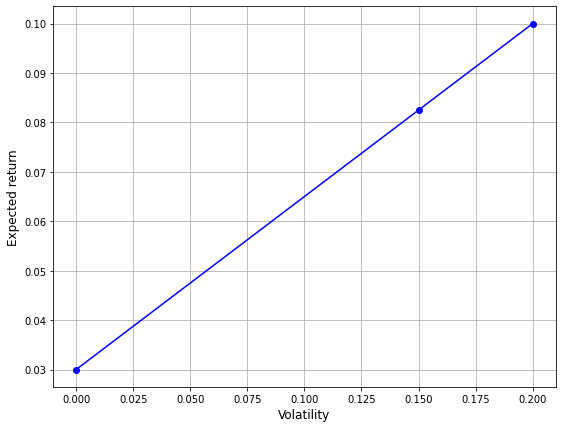
\includegraphics[width=0.6\linewidth]{cal}
    \end{center}
  \end{figure}
  \end{columns}
\end{frame}

\begin{frame}{Sharpe Ratio}
  \begin{itemize}
    \item The goal of an investor is to find the portfolio that generates the steepest possible line when combined with a risk-free investment. 
    \item  The slope of this line is called the \emph{Sharpe ratio}
      \begin{equation*}
        \mathcal{S} = (R_P - r_0) / \sigma_P
      \end{equation*}
      with $R_P$ and $\sigma_p$ portfolio expected return and risk, and $r_0$ the return of the risk-free asset.
    \item \emph{Sharpe ratio measures how much additional return we achieved for the additional risk we took on, relative to putting all our money in a risk-free asset}.
  \end{itemize}
\end{frame}

\begin{frame}{Sharpe Ratio as Optimization Criteria}
  \begin{itemize}
    \item Assume you want to achieve a certain level of return $R_{\textrm{target}}$ with your portfolio, what is the fraction $w_P$ of your wealth to place in the risky part of the portfolio ?
      \begin{equation*}
        \begin{gathered}
          ( 1 - w_P ) \cdot r_0 + w_P \cdot R_P = R_{\textrm{target}}\\
          w_P = \cfrac{( R_{\textrm{target}} – r_0)}{( R_P – r_0)}
        \end{gathered}
      \end{equation*}
    \item The corresponding risk is
      \begin{equation*}
        w_P\cdot \sigma_P = \left[\cfrac{( R_{\textrm{target}} – r_0)}{(R_P – r_0)}\right]\cdot \sigma_P
      \end{equation*}
    \item So if you want to minimize the portfolio risk you need to find:
      \begin{equation*}
        \min\left\{\left[\cfrac{(R_{\textrm{target}} – r_0)}{(R_P – r_0)}\right]\cdot \sigma_P\right\} = \min\left\{\cfrac{( R_{\textrm{target}} – r_0)}{\mathcal{S}}\right\}
      \end{equation*}
  \end{itemize}
\end{frame}

\begin{frame}{Sharpe Ratio as Optimization Criteria}
  \begin{itemize}     
    \item But $R_{\textrm{target}}$ and $r_0$ are fixed so minimizing the above ratio is equivalent to maximize the Sharpe ratio:
      \begin{equation*}
        \min\left\{\cfrac{( R_{\textrm{target}} – r_0)}{\mathcal{S}}\right\} \implies\max\left\{\mathcal{S}\right\}
      \end{equation*}
    \item \emph{The risky portfolio that maximizes the Sharpe ratio is the one that minimize the variance at the same time}.
    \item In other words, the optimization using the Sharpe ratio gives a portfolio that is on the minimum volatility efficient frontier, and gives the maximum return relative to putting all our money in the risk-free asset.
  \end{itemize}
\end{frame}

\begin{frame}{Portfolio Diversification}
  \begin{itemize}
  \item A security total risk can be divided into:
    \begin{itemize}
      \item \emph{unsystematic}, the risk portion peculiar to the company that can be diversified away;
      \item \emph{systematic}, the non-diversifiable portion that is related to the movement of the stock market and is therefore unavoidable.
    \end{itemize}
  \item \emph{Diversification} is a common topic in portfolio construction and allows to combine risky stocks so that the resulting portfolio is less risky than the sum of its components. 
  \item Unfortunately, perfect negative relationship between the returns is very rare in real world; however diversification will always reduce risk.
  \item For example assumng an equally weighted portfolio
    \begin{equation*}
      \sigma_P = \sqrt{0.5\sigma_1^2 + 0.5\sigma_2^2 + 2 \cdot 0.5\sigma_1 \cdot 0.5\sigma_2\cdot\rho_{12}} \le  0.5\sigma_1 + 0.5\sigma_2
    \end{equation*}
  \item The inequality holds unless $\rho_{12} = 1$, so in general, \emph{for risk, the whole is less than the sum of its parts}.
    \end{itemize}
\end{frame}

\begin{frame}{Linear Models}
  \begin{itemize}
    \item \emph{Linear models} can be used whenever a \emph{target variable} ($y$) can be described as a linear combination of one or more \emph{independent variables} ($X$)
      \begin{equation*}
        y = \beta_1 X_1 + \beta_2 X_2 + \ldots + \alpha
      \end{equation*}
    \item In such models it is mandatory to avoid \emph{collinearity} among the independent variables, which means each $X_i$ cannot be expressed as a linear combination of other $X_j$, i.e. they really must be independent !
    \item A model before becoming useful needs to be \emph{calibrated}: need to find the model parameter values such that it explains at its best real data.
    \item Calibration of a linear model can be done with a \emph{linear regression} using \emph{ordinary least squares} (OLS) technique.
    \item OLS algorithm determine the model parameters such that the following is minimized
      \begin{equation*}
        \min_{\beta,\alpha}\sum_i (y_i - \tilde{y}_i)^2
      \end{equation*}
      where $\tilde{y}$ is the $y$ value predicted by the model.
  \end{itemize}
\end{frame}

\begin{frame}{Linear Regeression}
  \begin{itemize}
  \item Calibration of a linear model can be done with a \emph{linear regression} using \emph{ordinary least squares} (OLS) technique.
  \item OLS algorithm determines the model parameters such that the following is minimized
    \begin{equation*}
      \min_{\beta,\alpha}\sum_i (y_i - \tilde{y}_i)^2
    \end{equation*}
    where $\tilde{y}$ is the $y$ value predicted by the model.
  \end{itemize}
  \begin{figure}[h]
    \begin{center}
      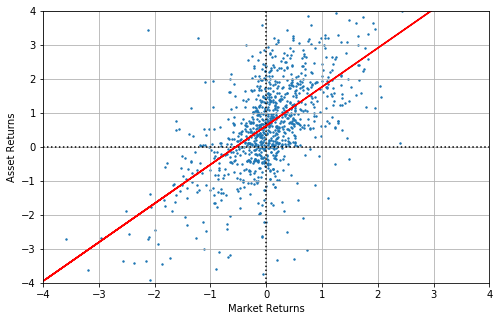
\includegraphics[width=0.45\linewidth]{linear_regression}
    \end{center}
  \end{figure}
\end{frame}

\begin{frame}{Capital Asset Pricing Model}
  \begin{itemize}
  \item The Capital Asset Pricing Model (CAPM) describes the relationship between expected return of assets and \emph{systematic risk} of the market.
  \item No measure of unsystematic risk appears in the risk premium for in the world of CAPM diversification has already eliminated it.
  \item In such a model, it is assumed a linear relationship between the expected return of any security (or portfolio) and the expected return of the \emph{market portfolio}. It is given by
    \begin{equation*}
      r_i = r_f + \beta_i(r_m-r_f)
    \end{equation*}
    where: $r_i$ is the expected return of the $i^{th}$ security, $r_f$ the risk-free rate (e.g. Treasury Bills rates), $r_m - r_f$ is the risk premium ($r_m$ denotes the market portfolio return e.g. an index like S\&P 500) and $\beta_i$ is a measure of $i^{th}$ asset volatility in relation to the overall market.
  \end{itemize}
\end{frame}

\begin{frame}{Capital Asset Pricing Model}
  \begin{itemize}
  \item The relationship between risk and expected return is called the security market line (SML).
  \item (Undervalued) No security can sell for long at prices low enough to yield more than its appropriate return on the SML; the security would then be very attractive compared with other securities of similar risk, and investors would bid its price up until its expected return fell to the appropriate position on the SML.
  \item (Overvalued) Conversely, investors would sell off any stock selling at a price high enough to put its expected return below its appropriate position. 
  \item The resulting reduction in price would continue until the stock’s expected return rose to the level justified by its systematic risk.The Capital Asset Pricing Model (CAPM) describes the relationship between expected return of assets and \emph{systematic risk} of the market.
  \end{itemize}
\end{frame}

\begin{frame}{Capital Asset Pricing Model}
  \begin{figure}[h]
    \begin{center}
      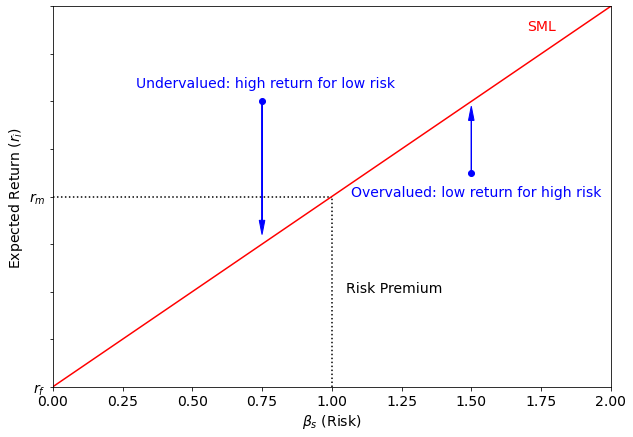
\includegraphics[width=0.45\linewidth]{sml}
    \end{center}
  \end{figure}
  CAPM $\beta$ can be estimated with the measurement of the slope of the \emph{regression line}, of the market vs individual stock return distribution.
\end{frame}


\begin{frame}{Regression in CAPM}
  \begin{itemize}
  \item The regressed coefficient estimates can be expressed as
    \begin{equation*}
      \beta \approx \cfrac{\textrm{cov}(X,y)}{\textrm {var}(X)}
    \end{equation*}
  \item Provides insights about how \emph{volatile}, or how risky, a stock is relative to the rest of the market.
  \item CAPM $\beta$ calculation helps investors understand whether a stock moves in the same direction as the rest of the market
    \begin{itemize}
      \item $\beta= 1.0$ stock price is perfectly correlated with the market;
      \item $\beta < 1.0$ ("defensive"), the security is theoretically less volatile than the market (i.e. provides lower returns, so it is less risky);
      \item $\beta > 1.0$, ("aggressive"), the assets price is more volatile than the market.
    \end{itemize}
  \item The point is to find stocks that have high $\beta$, and portfolios that have high $\alpha$. 
  \item High $\beta$ values mean that the stock fares better than index; $\alpha$ values above zero mean that your portfolio gives positive return no matter what the market does.
  \end{itemize}
\end{frame}

\begin{frame}{Multifactor Models}
  \begin{itemize}
  \item In its original formulation CAPM treats the market return as the only factor.
  \item Nevertheless a stock’s return can depend also on other macro-economic factors, such commodity prices, interest rates, economic growth (GDP).
    \begin{equation*}
      r_i = \alpha + \beta_1 f_1 + \beta_2 f_2 + \beta_3 f_3 + \ldots
    \end{equation*}
  \item Commonly used multi-factor models are \emph{Fama-French} and \emph{Barra} with their extensions.
  \end{itemize}
\end{frame}

\end{document}

